\documentclass[11pt,aspectratio=169]{beamer}

\usepackage[utf8]{inputenc}
\usepackage[T1]{fontenc}
\usepackage[spanish,es-tabla]{babel}
\usepackage{lmodern}
\usepackage[table]{xcolor}
\usepackage{booktabs}
\usepackage{tikz}
\usetikzlibrary{positioning, arrows.meta, fit, shapes.geometric, calc}
\usepackage[most]{tcolorbox}
\usepackage{microtype}
\usepackage{pifont}

\definecolor{accent}{HTML}{1F6FEB}
\definecolor{accent2}{HTML}{0A8754}
\definecolor{warn}{HTML}{D1351A}
\definecolor{bg}{HTML}{F6F8FA}
\definecolor{bgbox}{HTML}{EDF2F7}
\definecolor{rule}{HTML}{D0D7DE}
\definecolor{ink}{HTML}{1F2328}
\definecolor{muted}{HTML}{57606A}
\definecolor{good}{HTML}{1A7F37}

\usetheme{default}
\setbeamercolor{normal text}{fg=ink, bg=white}
\setbeamercolor{frametitle}{fg=accent, bg=white}
\setbeamercolor{title}{fg=ink}
\setbeamercolor{itemize item}{fg=accent}
\setbeamercolor{itemize subitem}{fg=accent}
\setbeamercolor{block title}{bg=bgbox, fg=accent}
\setbeamercolor{block body}{bg=bg, fg=ink}
\setbeamercolor{footline}{fg=muted}

\setbeamerfont{frametitle}{size=\Large, series=\bfseries}
\setbeamerfont{title}{size=\huge, series=\bfseries}

\setbeamertemplate{navigation symbols}{}
\setbeamertemplate{itemize item}{\raisebox{0.15ex}{\scriptsize\textbullet}}

\setbeamertemplate{frametitle}{%
  \nointerlineskip
  \vspace*{0.4em}
  \begin{beamercolorbox}[wd=\paperwidth, leftskip=0.6cm, rightskip=0.6cm]{frametitle}
    \insertframetitle\par
    \vspace*{0.15em}
    \textcolor{rule}{\rule{\dimexpr\paperwidth-1.2cm\relax}{0.4pt}}
  \end{beamercolorbox}
}

\setbeamertemplate{footline}{%
  \leavevmode%
  \hbox{%
    \begin{beamercolorbox}[wd=0.5\paperwidth, ht=2.5ex, dp=1ex, leftskip=0.6cm]{footline}
      \usebeamerfont{footline}\small TP3 · Perceptrones
    \end{beamercolorbox}%
    \begin{beamercolorbox}[wd=0.5\paperwidth, ht=2.5ex, dp=1ex, rightskip=0.6cm]{footline}
      \hfill\usebeamerfont{footline}\small\insertframenumber\,/\,\inserttotalframenumber
    \end{beamercolorbox}%
  }%
}

\newtcolorbox{insight}{
  enhanced, breakable,
  colback=bgbox, colframe=accent,
  boxrule=0pt, leftrule=4pt,
  arc=2pt, outer arc=0pt,
  left=8pt, right=8pt, top=4pt, bottom=4pt
}
\newtcolorbox{warning}{
  enhanced, breakable,
  colback=bgbox, colframe=warn,
  boxrule=0pt, leftrule=4pt,
  arc=2pt, outer arc=0pt,
  left=8pt, right=8pt, top=4pt, bottom=4pt
}
\newtcolorbox{takeaway}{
  enhanced, breakable,
  colback=accent2!8, colframe=accent2,
  boxrule=0pt, leftrule=4pt,
  arc=2pt, outer arc=0pt,
  left=8pt, right=8pt, top=4pt, bottom=4pt
}

\newcommand{\code}[1]{\texttt{\textcolor{accent}{#1}}}
\newcommand{\file}[1]{\texttt{\small #1}}
\newcommand{\ok}{\textcolor{good}{\ding{52}}}
\newcommand{\nok}{\textcolor{warn}{\ding{56}}}

\newcommand{\sectiondivider}[2]{%
  \begingroup
  \setbeamercolor{background canvas}{bg=accent}
  \begin{frame}[plain]
    \centering
    \vspace*{2cm}
    \color{white}
    {\fontsize{14}{16}\selectfont\bfseries Bloque #1}\\[1.2em]
    {\fontsize{32}{38}\selectfont\bfseries #2}\\[1.5em]
    \textcolor{white!75}{\rule{6cm}{0.4pt}}\\
  \end{frame}
  \endgroup
}

\title{TP3 — Perceptrones}
\subtitle{Resultados experimentales sobre tres ejercicios}
\author{}
\institute{Sistemas de Inteligencia Artificial · ITBA · 1Q 2026}
\date{}

\setbeamertemplate{title page}{%
  \begin{tikzpicture}[remember picture, overlay]
    \fill[accent] (current page.north west) rectangle ($(current page.south west) + (0.5,0)$);
    \foreach \x in {0,...,28} {
      \foreach \y in {0,...,16} {
        \fill[accent!18] ($(current page.north west) + (1.0 + 0.5*\x, -0.6 - 0.5*\y)$) circle (1pt);
      }
    }
  \end{tikzpicture}
  \vspace*{1.4cm}
  \begin{flushleft}
    \hspace*{1cm}{\fontsize{40}{46}\selectfont\bfseries\color{ink}TP3}\\[0.3em]
    \hspace*{1cm}{\fontsize{30}{36}\selectfont\bfseries\color{accent}Perceptrones}\\[0.6em]
    \hspace*{1cm}{\Large\color{muted}\inserttitle\hfill}\\
    \hspace*{1cm}{\large\color{muted}\insertsubtitle}\\[1.6em]
    \hspace*{1cm}{\color{muted}\insertinstitute}\\
  \end{flushleft}
}

\begin{document}

% ============= 1. Portada =============
{
\setbeamertemplate{footline}{}
\begin{frame}[plain]
  \titlepage
\end{frame}
}

% ===================================================================
\sectiondivider{Antes de los ejercicios}{Decisiones de diseño}

% ---- Slide D2: Función de activación (modificada) ----
\begin{frame}{Función de activación — \textbf{cuál y por qué}}
\small
\begin{tabular}{@{}p{0.32\linewidth}p{0.18\linewidth}p{0.46\linewidth}@{}}
\toprule
\textbf{Dónde} & \textbf{Cuál} & \textbf{Por qué} \\
\midrule
Ej 1 — distillation & sigmoide & Target en $[0,1]$ (probabilidad). La sigmoide naturalmente devuelve ese rango. \\
\rowcolor{accent2!10}
Ej 2 / Ej 3 — capas ocultas & \textbf{ReLU} & Gradiente fuerte y constante en zona positiva. No satura como tanh/sigmoide. Entrena rápido. \\
\rowcolor{accent2!10}
Ej 2 / Ej 3 — capa de salida & \textbf{softmax} & Clasificación multiclase: devuelve distribución de probabilidad sobre las 10 clases. \\
\bottomrule
\end{tabular}\\[0.6em]

\begin{insight}
\textbf{¿Qué es ``saturar''?} Una activación satura cuando la pendiente $f'(z)$ se aproxima a $0$ para entradas grandes en magnitud. Sigmoide y tanh saturan en sus extremos: el gradiente que llega a las capas previas se desvanece (\emph{vanishing gradient}) y la red deja de aprender.
\end{insight}

\begin{takeaway}
\textbf{ReLU $= \max(0, z)$}: derivada $1$ en zona positiva, $0$ en negativa. Sin saturación en su lado activo $\Rightarrow$ el gradiente fluye sin atenuarse a través de muchas capas. Es la activación estándar moderna para capas ocultas.
\end{takeaway}
\end{frame}

% ---- Slide D3: Inicialización (modificada: sin "regla del apunte" ni comentario al pie) ----
\begin{frame}{Inicialización de pesos — \textbf{cuál y por qué}}
\begin{itemize}\setlength\itemsep{0.2em}\small
  \item \textbf{¿Por qué no cero?} Si todas las neuronas arrancan iguales, hacen exactamente lo mismo en cada capa. El gradiente las mueve igual y \emph{nunca se diferencian} (problema de simetría).
  \item \textbf{¿Por qué pequeños?} Pesos grandes saturan las activaciones (especialmente sigmoide/tanh): la salida queda en zonas planas, el gradiente es casi cero, la red no aprende.
\end{itemize}
\vspace{0.6em}

\centering\small
\begin{tabular}{@{}p{0.18\linewidth}p{0.34\linewidth}p{0.44\linewidth}@{}}
\toprule
\textbf{Esquema} & \textbf{Distribución} & \textbf{Cuándo lo usamos} \\
\midrule
\textbf{He}      & $\mathcal{N}\!\left(0, \sqrt{2/\text{fan\_in}}\right)$ & Capas con \textbf{ReLU}: compensa que ReLU descarta la mitad del input. \\
\textbf{Xavier}  & $\mathcal{N}\!\left(0, \sqrt{1/\text{fan\_in}}\right)$ & Capas con \textbf{tanh / sigmoide / softmax}: mantiene varianza balanceada. \\
\textbf{Uniforme} & $\mathcal{U}[-0.1, +0.1]$                            & Perceptrón simple del Ej 1 (sin propagación profunda). \\
\bottomrule
\end{tabular}
\end{frame}

% ---- Slide D4: Optimizador (ok) ----
\begin{frame}{Optimizador — \textbf{cuál y por qué}}
\textbf{La clase introduce gradiente descendente clásico} (SGD); Momentum y Adam son extensiones modernas. Comparamos los tres.\\[0.6em]

\begin{itemize}\setlength\itemsep{0.25em}\small
  \item \textbf{SGD vanilla}: $w \leftarrow w - \eta \cdot \nabla L$. Lo más simple. Funciona pero es lento, especialmente en superficies con valles alargados.
  \item \textbf{Momentum} ($\beta = 0.9$): acumula \emph{velocidad} en la dirección del gradiente. Atraviesa valles sin oscilar.
  \item \textbf{Adam} ($\beta_1 = 0.9$, $\beta_2 = 0.999$, $\varepsilon = 10^{-8}$): combina momentum con \emph{learning rate adaptativo por parámetro}. El PDF de optimizadores lo califica textual como \emph{``muy usado en la práctica''} (defaults idénticos al paper Kingma \& Ba 2015).
\end{itemize}
\vspace{0.6em}

\begin{takeaway}
\textbf{Resultado en Ej 2} (sweep Fase 1.2, K-fold=5): \\
\textbf{Adam} 96.74\% (best\_ep=7) \quad $\approx$ \quad Momentum 96.34\% \quad $\gg$ \quad SGD 94.81\% (no convergió en 50 epochs).\\[0.2em]
\textbf{Elegimos Adam} por convergencia más rápida y resultado igual o mejor.
\end{takeaway}
\end{frame}

% ---- Slide D5: Learning rate (modificada: nombres de fases + comentario simplificado) ----
\begin{frame}{Learning rate — \textbf{cuál y por qué}}
\textbf{Recomendación de la clase:} learning rate \emph{pequeño}; probar varios órdenes de magnitud y mapear cómo afectan a la convergencia.\\[0.5em]

\begin{itemize}\setlength\itemsep{0.15em}\small
  \item \textbf{Demasiado grande} → la red oscila o diverge.
  \item \textbf{Demasiado chico} → no converge en tiempo razonable.
\end{itemize}
\vspace{0.6em}

\textbf{Experimentación en dos pasos} (Ej 2):\\[0.3em]

\centering\small
\begin{tabular}{@{}p{0.30\linewidth}p{0.36\linewidth}p{0.28\linewidth}@{}}
\toprule
\textbf{Etapa} & \textbf{Valores barridos} & \textbf{Resultado} \\
\midrule
\textbf{Fase 1 exploratoria} (k=1)  & $\{10^{-4}, 5\!\cdot\!10^{-4}, 10^{-3}, 5\!\cdot\!10^{-3}, 10^{-2}\}$ & $10^{-3}$ ganó \\
\rowcolor{accent2!10}
\textbf{Fase 2 validación} (k=5) & $\{10^{-4}, 10^{-3}, 10^{-2}, 0.1, 10\}$ con extremos & $10^{-3}$ confirmado \\
\bottomrule
\end{tabular}\\[0.6em]

\begin{takeaway}
\textbf{Elegimos $lr = 10^{-3}$ con Adam.}
\end{takeaway}
\end{frame}

% ---- NUEVA: LR sweep tabla Fase 1 (de docs/lr_sweep_conclusion.md) ----
\begin{frame}{Learning rate — Fase 1 exploratoria (k=1)}
\centering\small
\begin{tabular}{@{}lrrrrl@{}}
\toprule
\textbf{LR} & \textbf{val\_acc} & \textbf{macro\_f1} & \textbf{best\_ep} & \textbf{total\_ep} & \textbf{Comportamiento} \\
\midrule
\rowcolor{accent2!15}
\textbf{0.001} & \textbf{96.74\%} & \textbf{0.863} & \textbf{7} & \textbf{18} & $\checkmark$ Óptimo \\
0.0005 & 96.54\% & 0.864 & 17 & 28 & Lento \\
0.0001 & 96.22\% & 0.861 & 47 & 50 & No converge \\
0.005  & 96.02\% & 0.857 & 4  & 15 & Overshoot moderado \\
0.01   & 95.30\% & 0.850 & 2  & 13 & Overshoot fuerte \\
\bottomrule
\end{tabular}\\[0.8em]

\raggedright\small
\textbf{Tres criterios convergen en $lr = 10^{-3}$:}
\begin{itemize}\setlength\itemsep{0.1em}
  \item Máximo claro de \textbf{val\_acc} (forma de parábola).
  \item Convergencia rápida: \textbf{best\_epoch=7} vs 47 con $10^{-4}$.
  \item Sin overshoot ($lr \geq 5\!\cdot\!10^{-3}$ corta a las 2-4 épocas, demasiado temprano).
\end{itemize}
\end{frame}

% ---- NUEVA: LR sweep tabla Fase 2 (de docs/lr_sweep_conclusion.md) ----
\begin{frame}{Learning rate — Fase 2 validación (k=5)}
\centering\small
\begin{tabular}{@{}lrrl@{}}
\toprule
\textbf{LR} & \textbf{val\_acc} & \textbf{best\_ep} & \textbf{Tiempo / Comportamiento} \\
\midrule
\rowcolor{accent2!15}
\textbf{0.001} & \textbf{96.22\%} & \textbf{4.6} & \textbf{449 s} \\
0.0001 & 95.79\% & 31.6 & 1390 s ($3.1\times$ más lento) \\
0.01   & 94.71\% & 4.6  & 455 s, overshoot \\
0.1    & 29.00\% & 7.2  & \textcolor{warn}{divergencia catastrófica} \\
10     & 12.48\% & 11.6 & \textcolor{warn}{NaN, loss explota} \\
\bottomrule
\end{tabular}\\[0.8em]

\begin{warning}
\textbf{Extremos catastróficos confirmados.} Con $lr=10$ la red queda en accuracy random (12\%, equivalente a $1/10$ clases). Con $lr=0.1$ también diverge.
\end{warning}
\vspace{0.4em}

\begin{takeaway}
\textbf{$lr = 10^{-3}$ confirmado por dos sweeps independientes.} Robusto frente a la varianza del K-fold.
\end{takeaway}
\end{frame}

% ---- Slide D7: Convergencia y bias (modificada según notas) ----
\begin{frame}{Convergencia y bias — \textbf{decisiones de implementación}}
\small
\begin{columns}[T]
\column{0.50\linewidth}
\textbf{Criterio de convergencia}\\[0.3em]

\begin{tabular}{@{}p{0.16\linewidth}p{0.78\linewidth}@{}}
\toprule
\textbf{Ej} & \textbf{Criterio} \\
\midrule
Ej 1 & $\varepsilon$ absoluto sobre MSE de train (\emph{regla del apunte} para perceptrón simple). Corta cuando $\text{mse} < \varepsilon$. \\
\rowcolor{accent2!10}
Ej 2/3 & \textbf{Early stopping} sobre \code{val\_loss} con \code{patience}=10. \\
\bottomrule
\end{tabular}\\[0.5em]

\begin{insight}
Early stopping detecta overfitting que $\varepsilon$ solo no detecta.
\end{insight}

\column{0.50\linewidth}
\textbf{Manejo del bias}\\[0.3em]

\begin{itemize}\setlength\itemsep{0.2em}
  \item \textbf{Bias trick}: agregamos columna de 1's al input de cada capa $\Rightarrow$ pesos con shape \code{(n\_out, n\_in+1)}. El bias es un peso más, se actualiza con la misma regla de gradiente.
\end{itemize}
\end{columns}
\end{frame}

% ===================================================================
\sectiondivider{1 / 3}{Ej 1 — Knowledge Distillation}

% ============= Ej 1 — El problema (modificada: Ground truth -> Criterio de evaluación) =============
\begin{frame}{Ej 1 — El problema}
\textbf{Knowledge distillation:} replicar la salida del BigModel pre-entrenado con un TinyModel (perceptrón simple).\\[0.6em]

\begin{columns}[T]
\column{0.55\linewidth}
\textbf{Datos:} \file{fraud\_dataset.csv}\\
9 features (amount, session, account\_age, ...)\\[0.4em]

\textbf{Target de entrenamiento:}\\
\code{big\_model\_fraud\_probability} (continuo en $[0,1]$).\\[0.4em]

\textbf{Criterio de evaluación:}\\
\code{flagged\_fraud} (binaria 0/1).

\column{0.45\linewidth}
\begin{warning}
\textbf{Regla del enunciado:}\\ \code{flagged\_fraud} \emph{nunca} se usa para entrenar. Solo para métricas operativas (precision, recall, F1) post-hoc.
\end{warning}
\vspace{0.6em}

\textbf{Salida esperada en $[0,1]$} $\Rightarrow$ activación sigmoide.
\end{columns}
\end{frame}

% ============= NUEVA: Análisis del dataset — tres reglas =============
\begin{frame}{Ej 1 — Análisis del dataset: tres reglas determinísticas}
\textbf{Antes de entrenar:} la exploración del dataset reveló \textbf{umbrales duros} en tres features que separan las clases.\\[0.4em]

\begin{center}\footnotesize
\fbox{\parbox{0.92\linewidth}{\centering
\code{amount\_usd > 500} $\;\vee\;$ \code{quantity\_purchased $\geq$ 10} $\;\vee\;$ \code{items\_viewed\_before\_purchase $\geq$ 15}
}}
\end{center}
\vspace{0.3em}

\centering\footnotesize
\begin{columns}[T]
\column{0.44\linewidth}
\textbf{Aporte individual:}\\[0.2em]
\begin{tabular}{@{}lrrr@{}}
\toprule
\textbf{Regla} & \textbf{Matches} & \textbf{TP} & \textbf{FP} \\
\midrule
\code{amount\_usd > 500}              & 199 & 199 & 0 \\
\code{quantity $\geq$ 10}             & 524 & 524 & 0 \\
\code{items\_viewed $\geq$ 15}        & 490 & 490 & 0 \\
\bottomrule
\end{tabular}\\[0.2em]
\textcolor{muted}{\scriptsize Las tres juntas marcan \textbf{695 filas únicas}.}

\column{0.54\linewidth}
\textbf{OR como predictor (\code{simple\_prediction}):}\\[0.2em]
\begin{tabular}{@{}lcc@{}}
\toprule
 & \multicolumn{2}{c}{\textbf{Predicción}} \\
\cmidrule(lr){2-3}
 & 1 (fraude) & 0 (no fraude) \\
\midrule
Real 1 (fraude)    & \textcolor{good}{\textbf{TP=695}} & \textcolor{warn}{\textbf{FN=174}} \\
Real 0 (no fraude) & \textcolor{warn}{\textbf{FP=0}}   & \textcolor{good}{\textbf{TN=6631}} \\
\bottomrule
\end{tabular}\\[0.3em]

\begin{tabular}{@{}lr@{}}
Accuracy  & \textbf{97.68\%} \\
Precision & \textbf{100.00\%} \\
Recall    & \textbf{79.98\%} \\
\end{tabular}
\end{columns}
\end{frame}

% ============= NUEVA: Conclusión del análisis (cuadrito 80%) =============
\begin{frame}{Ej 1 — Conclusión del análisis del dataset}
\centering
\vspace*{0.4cm}

\begin{insight}
\large
\textbf{El 80\% del fraude se etiqueta correctamente con tres \code{if}, sin un solo falso positivo.}\\[0.5em]
\textbf{El 20\% restante (174 casos)} es el verdadero desafío del perceptrón: son fraudes que respetan los tres umbrales y solo se detectan combinando features continuas.
\end{insight}
\vspace{0.8em}

\raggedright\small\textbf{Implicancias para el TinyModel:}
\begin{itemize}\setlength\itemsep{0.05em}
  \item \textbf{Línea de base}: el modelo debe igualar a las tres reglas (recall $\geq 80\%$).
  \item \textbf{Valor agregado}: se mide en cuántos de los 174 fraudes ``sutiles'' logra recuperar.
  \item \textbf{Lineal vs no-lineal}: las discontinuidades duras (saltos $\sim$6\%$\to$100\%) son imposibles para una recta — el perceptrón no-lineal debe mostrar ventaja.
\end{itemize}
\end{frame}

% ============= MSE comparison (ok) =============
\begin{frame}{Ej 1 — Lineal vs No-Lineal: MSE de distillation}
\textbf{Mismo dataset, K-fold = 5 estratificado, mismas features.} Diferencia: presencia de la sigmoide.\\[0.8em]

\centering
\begin{tabular}{@{}lr@{}}
\toprule
\textbf{Modelo} & \textbf{MSE test (mean $\pm$ std)} \\
\midrule
Lineal (Adaline)        & $0.0266 \pm 0.0008$ \\
\rowcolor{accent2!15}
\textbf{No-Lineal (sigmoide)} & $\boldsymbol{0.0110 \pm 0.0004}$ \quad ($\boldsymbol{-59\%}$) \\
\bottomrule
\end{tabular}\\[1.2em]

\begin{insight}
\textbf{¿Por qué la sigmoide gana tan claro?}\\
El target es una probabilidad acotada en $[0,1]$. La sigmoide \emph{naturalmente} mapea su salida a ese rango. El lineal puede producir valores fuera de $[0,1]$ y el MSE penaliza fuerte esa salida fuera de dominio.
\end{insight}
\end{frame}

% ============= Threshold sweep (titulo cambiado) =============
\begin{frame}{Ej 1 — Pruebas sobre threshold}
\centering
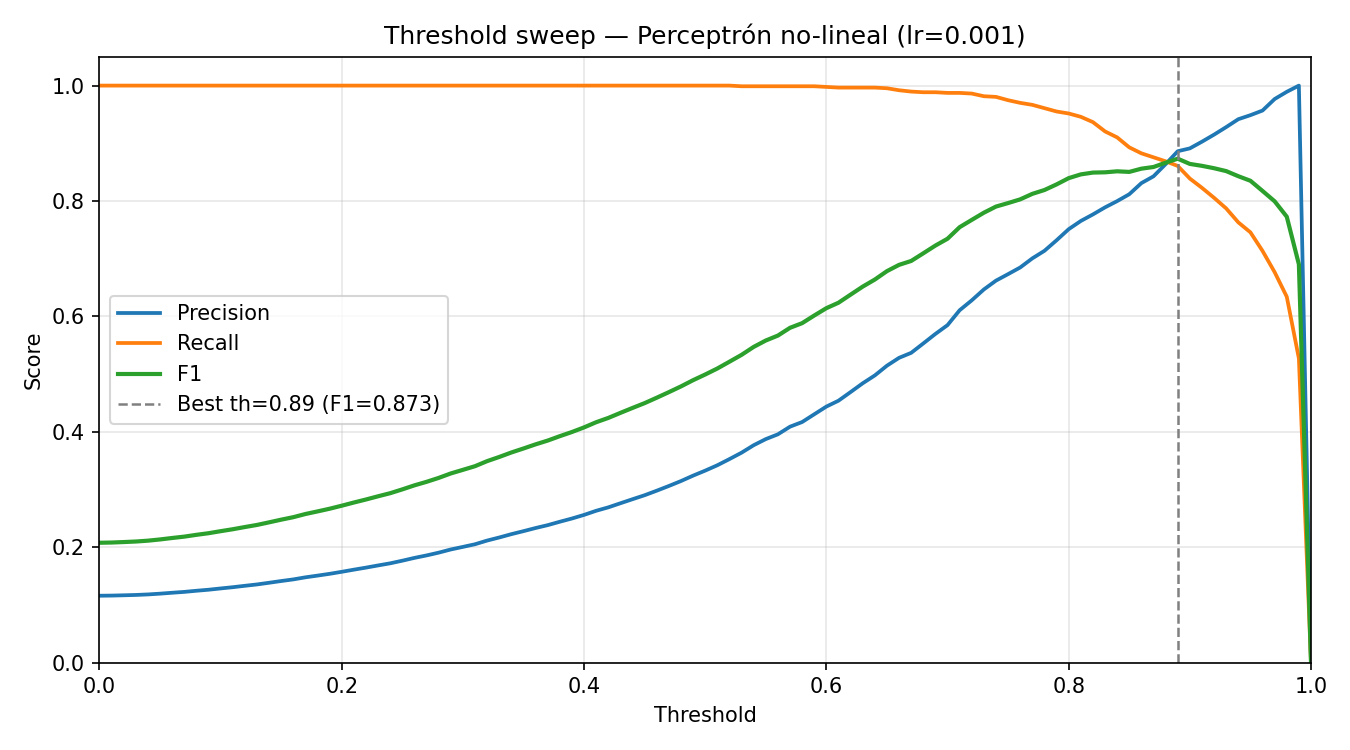
\includegraphics[width=0.62\linewidth]{../../ejercicio1/nonlinear_perceptron/analisis_outputs/threshold_sweep.png}\\[0.4em]

\begin{insight}
\textbf{Óptimo por F1: threshold = 0.89.}\\
Precision \(0.886\), recall \(0.861\), F1 \(0.873\), accuracy \(0.971\).
\end{insight}
\end{frame}

% ============= Recomendación (sin columna "Caso de uso", sin comentario "El modelo entrega scores") =============
\begin{frame}{Ej 1 — Recomendación de umbral}
\textbf{La elección depende del costo asimétrico falso positivo / falso negativo.}\\[0.8em]

\centering\small
\begin{tabular}{@{}lcccc@{}}
\toprule
\textbf{Threshold} & \textbf{Precision} & \textbf{Recall} & \textbf{F1} & \textbf{FP} \\
\midrule
0.50 (default)     & 0.333 & 1.000 & 0.499 & 1743 \\
\rowcolor{accent2!15}
\textbf{0.89} (óptimo F1) & \textbf{0.886} & \textbf{0.861} & \textbf{0.873} & \textbf{96} \\
0.95               & 0.949 & 0.746 & 0.835 & 35   \\
0.99               & 1.000 & 0.527 & 0.690 & 0    \\
\bottomrule
\end{tabular}
\end{frame}

% ===================================================================
\sectiondivider{2 / 3}{Ej 2 — Clasificación de dígitos}

% ============= Problema Ej2 (ok) =============
\begin{frame}{Ej 2 — El problema}
\textbf{Clasificación multiclase de dígitos manuscritos (0--9).}\\[0.6em]

\begin{columns}[T]
\column{0.5\linewidth}
\textbf{Datos:}
\begin{itemize}
  \item Train: \file{digits.csv} (12.449 muestras)
  \item Test: \file{digits\_test.csv} (2.498)
\end{itemize}
Cada muestra: vector de 784 floats $\in [0,1]$ (28$\times$28 flatten).

\column{0.5\linewidth}
\textbf{Arquitectura final:}
\begin{itemize}
  \item Input: 784
  \item Hidden 1: 100 (ReLU)
  \item Hidden 2: 50 (ReLU)
  \item Output: 10 (Softmax)
\end{itemize}
\end{columns}
\vspace{0.6em}

\begin{warning}
\textbf{Regla:} el test set se evalúa una sola vez al final. \\
Búsqueda de hiperparámetros sólo sobre \code{digits.csv}.
\end{warning}
\end{frame}

% ============= Workflow (titulo cambiado a "Fases de experimentación") =============
\begin{frame}{Ej 2 — Fases de experimentación}
\centering
\begin{tikzpicture}[
  every node/.style={font=\small},
  phase/.style={
    draw=accent, fill=bg, rounded corners=3pt,
    minimum width=3.4cm, minimum height=1.4cm, align=center
  },
  result/.style={
    draw=accent2, fill=accent2!10, rounded corners=3pt,
    minimum width=3.4cm, minimum height=1.4cm, align=center
  },
  arrow/.style={-{Latex[length=3mm]}, accent, very thick}
]
  \node[phase] (f1) {\textbf{Fase 1}\\\footnotesize k\_folds=1\\\footnotesize arch \(\to\) opt \(\to\) LR \(\to\) batch};
  \node[result, right=1.2cm of f1] (base) {\textbf{base.json}\\\footnotesize ganador\\\footnotesize consolidado};
  \node[phase, right=1.2cm of base] (f2) {\textbf{Fase 2}\\\footnotesize k\_folds=5\\\footnotesize one-at-a-time};
  \node[result, below=0.6cm of base] (final) {\textbf{final\_eval}\\\footnotesize digits\_test.csv\\\footnotesize (UNA sola vez)};

  \draw[arrow] (f1) -- (base);
  \draw[arrow] (base) -- (f2);
  \draw[arrow] (f2.south) -- ++(0,-0.3) -| (final.east);
  \draw[arrow, dashed] (base.south) -- (final.north);
\end{tikzpicture}\\[0.6em]

\begin{insight}
\textbf{Fase 1:} sweeps secuenciales para reducir el espacio de búsqueda. \\
\textbf{Fase 2:} K-fold=5 para validar la elección con comparativas robustas.
\end{insight}
\end{frame}

% ============= NUEVA: Sweep arquitectura — tabla de seccion 6 de decisiones_y_backing_teorico.md =============
\begin{frame}{Ej 2 — Sweep de arquitectura}
\centering\footnotesize
\begin{tabular}{@{}lcl@{}}
\toprule
\textbf{Arquitectura} & \textbf{val\_acc} & \textbf{Comentario} \\
\midrule
\rowcolor{accent2!15}
\textbf{[784, 100, 50, 10]}        & \textbf{96.74\% / 96.22\%} & \textbf{Ganador} por parsimonia \\
$[784, 128, 64, 10]$               & 96.86\% / —                 & Empate técnico ($\Delta < 0.4\%$) \\
$[784, 200, 100, 10]$ (\emph{wider})  & — / 96.39\%              & \textcolor{warn}{$-$0.48 pp test}, $3.6\times$ más lento \\
$[784, 100, 50, 25, 10]$ (\emph{deeper}) & — / 96.20\%           & Empate \\
$[784, 30, 10]$ (\emph{shallow})      & — / 95.15\%              & Subajustado \\
\bottomrule
\end{tabular}\\[0.8em]

\begin{takeaway}
\textbf{Decisión por parsimonia (regla de Occam):} cuando dos arquitecturas rinden igual dentro del desvío, gana la más simple/rápida. \textbf{Wider} confirma empíricamente la curva U del PDF de regularización: aumentar capacidad sin más datos $\Rightarrow$ overfitting (mejor val, peor test).
\end{takeaway}
\end{frame}

% ============= NUEVA: Sweep optimizador — tabla de seccion 3 de decisiones_y_backing_teorico.md =============
\begin{frame}{Ej 2 — Sweep de optimizador}
\centering\footnotesize
\begin{tabular}{@{}lccl@{}}
\toprule
\textbf{Optimizador} & \textbf{val\_acc} & \textbf{best\_ep} & \textbf{Comentario} \\
\midrule
\rowcolor{accent2!15}
\textbf{Adam} ($\alpha=10^{-3}$)        & \textbf{96.74\%} & \textbf{7}  & \textbf{Ganador} \\
Momentum ($\beta = 0.9$)                 & 96.34\%          & 18          & Converge más lento \\
SGD vanilla                              & 94.81\%          & 48          & No convergió en 50 epochs \\
\bottomrule
\end{tabular}\\[0.8em]

\begin{takeaway}
\textbf{Adam gana por convergencia más rápida y resultado igual o mejor.} El PDF de optimizadores lo califica textual como \emph{``muy usado en la práctica''} (defaults idénticos al paper Kingma \& Ba 2015). Momentum queda dentro del desvío; SGD claramente atrás sin aceleración.
\end{takeaway}
\end{frame}

% ============= Curvas (ok) =============
\begin{frame}{Ej 2 — Curvas de aprendizaje del modelo base (K=5)}
\centering
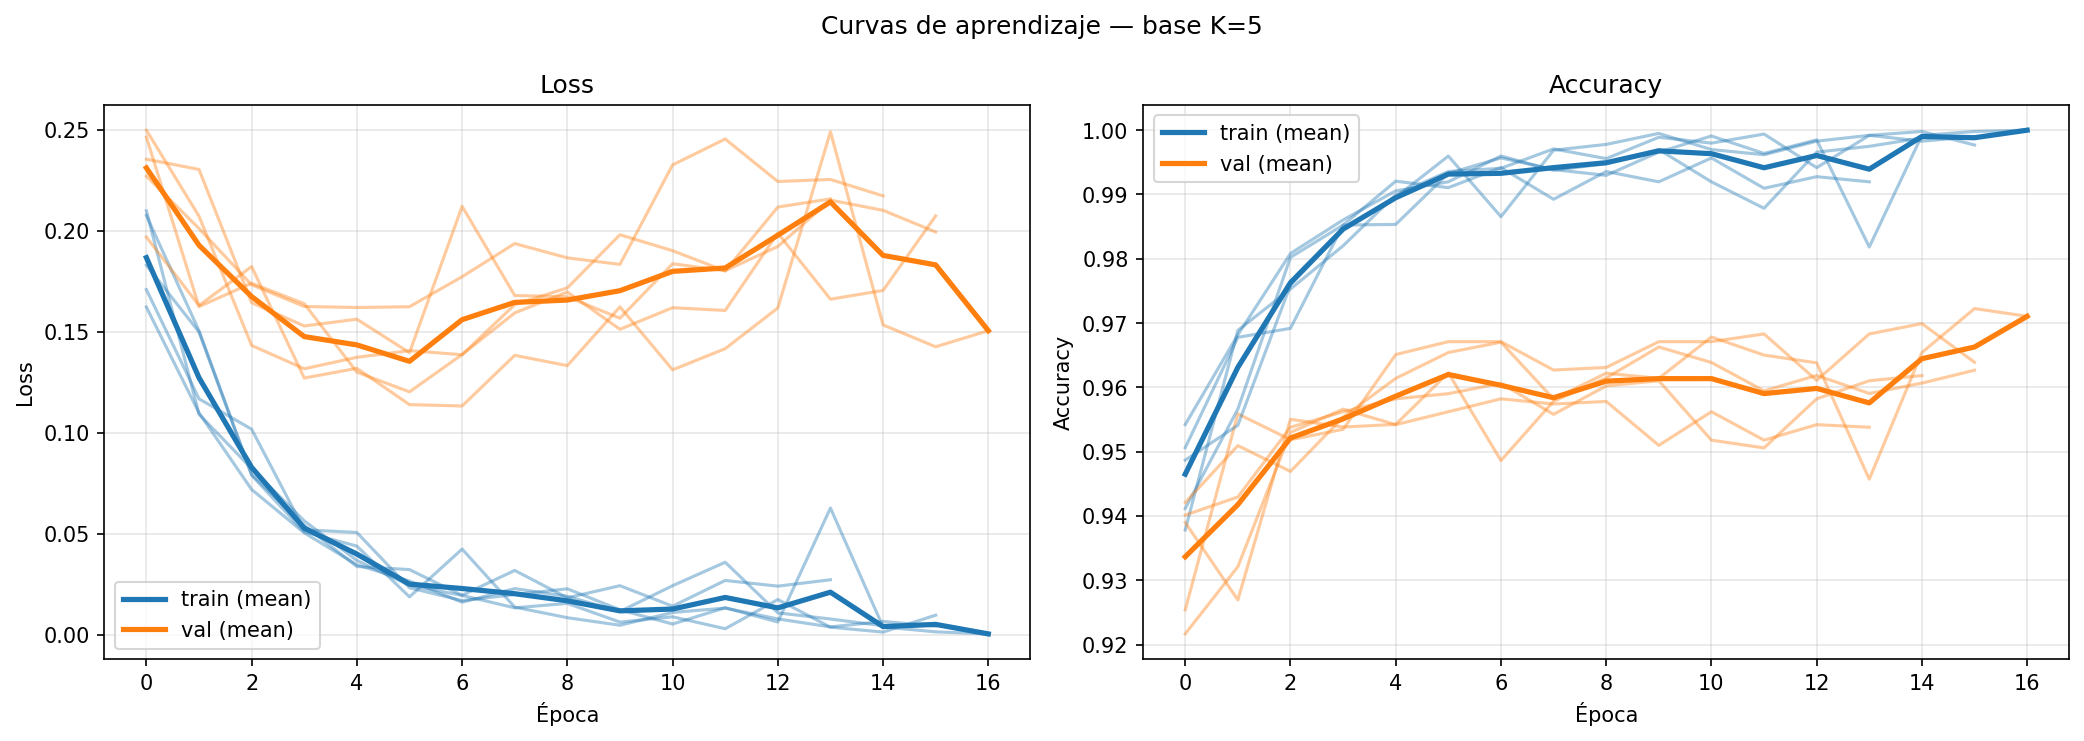
\includegraphics[width=0.78\linewidth]{../../ejercicio2/presentacion/01_curvas_aprendizaje_base.png}\\[0.3em]

\textbf{Convergencia limpia} en $\sim 5$ epochs. Train y validación bajan juntos: \textbf{sin overfitting visible}.
\end{frame}

% ============= Matriz base (ok) =============
\begin{frame}{Ej 2 — Matriz de confusión del base (val K=5)}
\centering
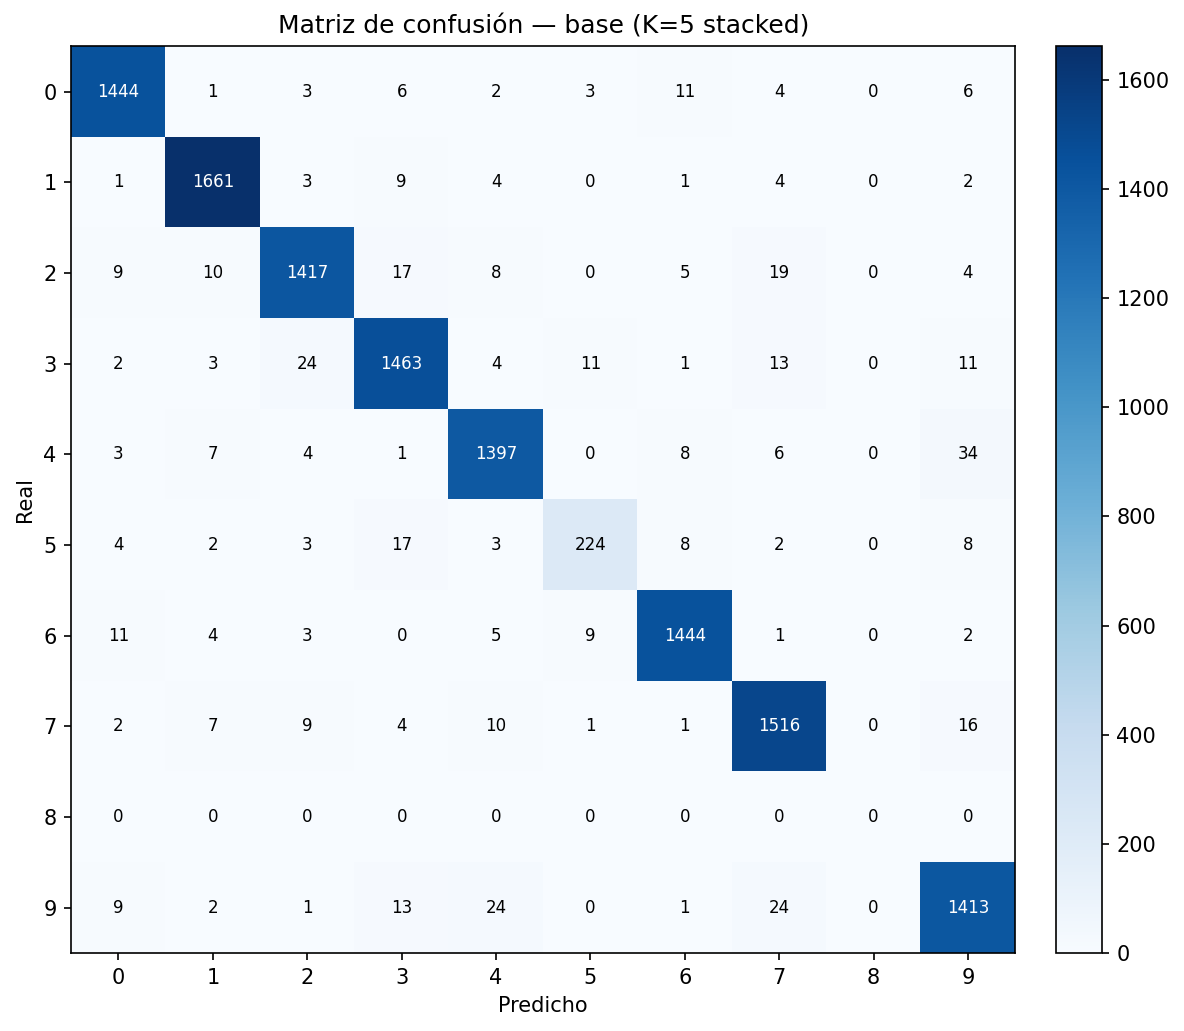
\includegraphics[width=0.38\linewidth]{../../ejercicio2/presentacion/04_confusion_matrix_base.png}\\[0.2em]

\begin{warning}
\textbf{Diagonal limpia para 9 de 10 clases. La clase 8 colapsa} (precision = recall = 0). $\Rightarrow$ Hint: algo raro pasa con la distribución de los datos.
\end{warning}
\end{frame}

% ============= Final eval (ok) =============
\begin{frame}{Ej 2 — Final eval: el cachetazo}
\centering
\vspace{0.3em}
\huge
val K-fold=5: \textbf{96.22\%}\\[0.4em]
\textcolor{muted}{$\downarrow$}\\[0.4em]
test (digits\_test.csv): \textcolor{warn}{\textbf{86.30\%}}\\[0.8em]
\Large \textbf{Drop de 10 puntos porcentuales.}\\[0.8em]

\normalsize
\begin{warning}
\textbf{Distribution shift, no underfitting.} El modelo está bien — los datos no se parecen.
\end{warning}
\end{frame}

% ============= Matriz final (ok) =============
\begin{frame}{Ej 2 — Matriz de confusión sobre digits\_test.csv}
\centering
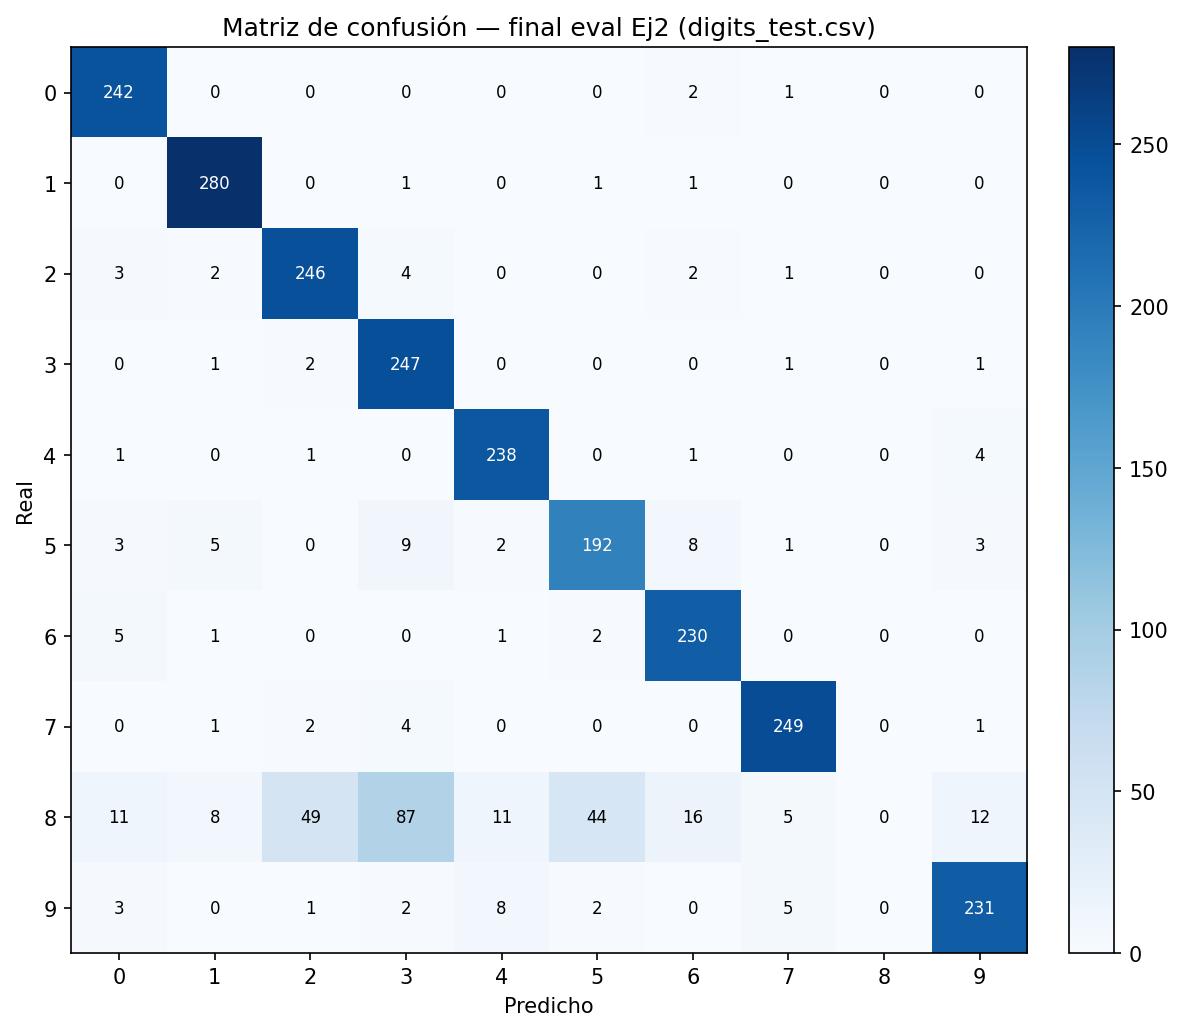
\includegraphics[width=0.38\linewidth]{../../ejercicio2/presentacion/08_confusion_matrix_final.png}\\[0.2em]

\begin{takeaway}
\textbf{Shift, no falta de capacidad:} confusiones distribuidas. $\Rightarrow$ \textbf{Más datos}, no más modelo. Eso es lo que el Ej 3 provee.
\end{takeaway}
\end{frame}

% ===================================================================
\sectiondivider{3 / 3}{Ejercicio 3 — Conclusiones}

% ============= Hipótesis y plan (modificada: "Pack C" -> "Se emplea regularizacion...", sin comentario) =============
\begin{frame}{Ej 3 — Hipótesis y plan}
\textbf{Hipótesis:} el techo del Ej 2 es por distribution shift, no por falta de capacidad.\\[0.6em]

\textbf{Plan secuencial:}
\begin{enumerate}
  \item \textbf{Más datos.} Concatenar \code{more\_digits.csv} (15.742 muestras adicionales). Si llega a $\geq 0.98$, listo.
  \item \textbf{Se emplea regularización} (L2, dropout, augmentation gaussiana, lr scheduling) y combinaciones.
  \item \textbf{Capacidad.} Si nada llega, probar \code{arch\_wider}.
\end{enumerate}
\end{frame}

% ============= Movimiento dominó (ok) =============
\begin{frame}{Ej 3 — El movimiento dominó}
\centering
\Huge
val K=5: \(96.22\% \to 97.06\%\)\\[0.4em]
test: \textcolor{warn}{\(86.30\%\)} \(\to\) \textcolor{accent2}{\(\boldsymbol{96.36\%}\)}\\[1em]

\Large\textbf{+10 puntos porcentuales en test.}\\
\large\textbf{\textcolor{muted}{Cero cambios al modelo. Solo más datos.}}\\[1em]

\normalsize
\begin{takeaway}
\textbf{Macro F1: $0.857 \to 0.959$.}\\
La clase 8 que estaba colapsada en Ej 2 ahora se predice correctamente. Más datos cubrieron el agujero de cobertura. Confirma la hipótesis del shift.
\end{takeaway}
\end{frame}

% ============= MOVED: Matriz de confusión del ganador (estaba después; ahora justo después del dominó) =============
\begin{frame}{Ej 3 — Matriz de confusión del ganador (test)}
\centering
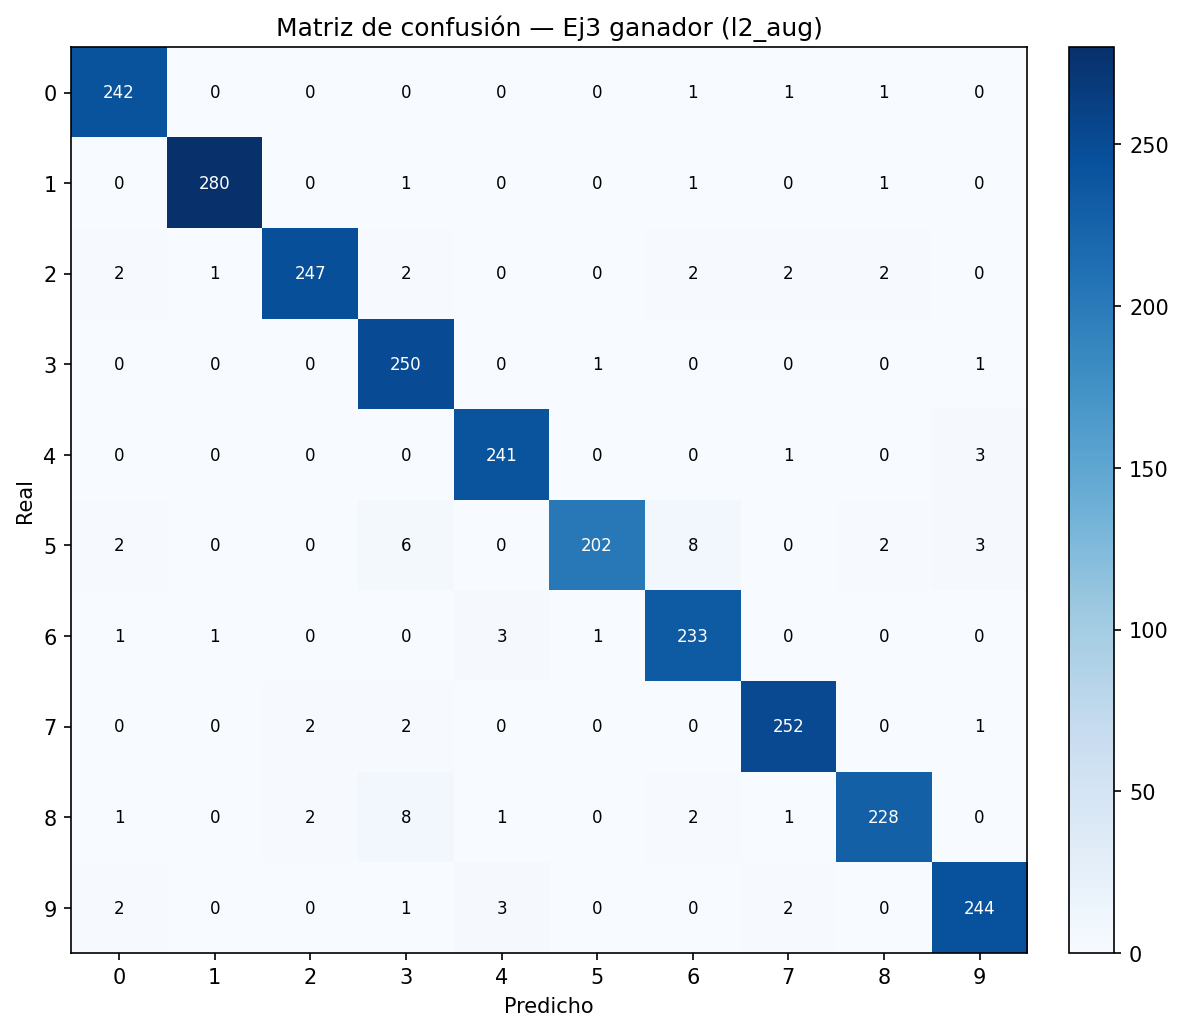
\includegraphics[width=0.36\linewidth]{../../ejercicio3/presentacion/02_confusion_matrix_ej3.png}\\[0.3em]

\begin{takeaway}
\textbf{La clase 8 que estaba colapsada en Ej 2 ahora se predice correctamente.} La diagonal está mucho más limpia, los errores residuales se reparten — síntoma de que ya no hay un agujero específico de cobertura, sino limitaciones globales del modelo.
\end{takeaway}
\end{frame}

% ============= Resultados (titulo cambiado de "Tabla Pack C" a "Resultados") =============
\begin{frame}{Ej 3 — Resultados}
\centering
\small
\begin{tabular}{@{}lrrr@{}}
\toprule
\textbf{Config} & \textbf{val K=5} & \textbf{test} & \textbf{$\Delta$ vs base\_extra} \\
\midrule
base\_extra\_data            & 0.9706 & 0.9636 & --- (referencia) \\
\quad +\,L2 (1e-4)            & 0.9758 & 0.9656 & $+0.20$ pp \\
\quad +\,dropout (p=0.2)      & 0.9750 & 0.9628 & $-0.08$ pp \\
\quad +\,L2 + dropout         & 0.9772 & 0.9604 & $-0.32$ pp \\
\rowcolor{accent2!15}
\textbf{\quad +\,L2 + aug ($\sigma=0.05$)} & \textbf{0.9760} & \textbf{0.9688} & \(\boldsymbol{+0.52}\)\textbf{ pp} \\
\quad +\,L2 + aug + dropout   & 0.9768 & 0.9656 & $+0.20$ pp \\
\quad +\,wider + L2 + aug     & 0.9777 & 0.9640 & $+0.04$ pp \\
\bottomrule
\end{tabular}\\[0.8em]

\textbf{Ganador:} L2 + augmentation gaussiana ($\sigma=0.05$) $\to$ \textbf{96.88\% en test}.
\end{frame}

% ============= Comparación visual (ok) =============
\begin{frame}{Ej 3 — Comparación visual con Ej 2}
\centering
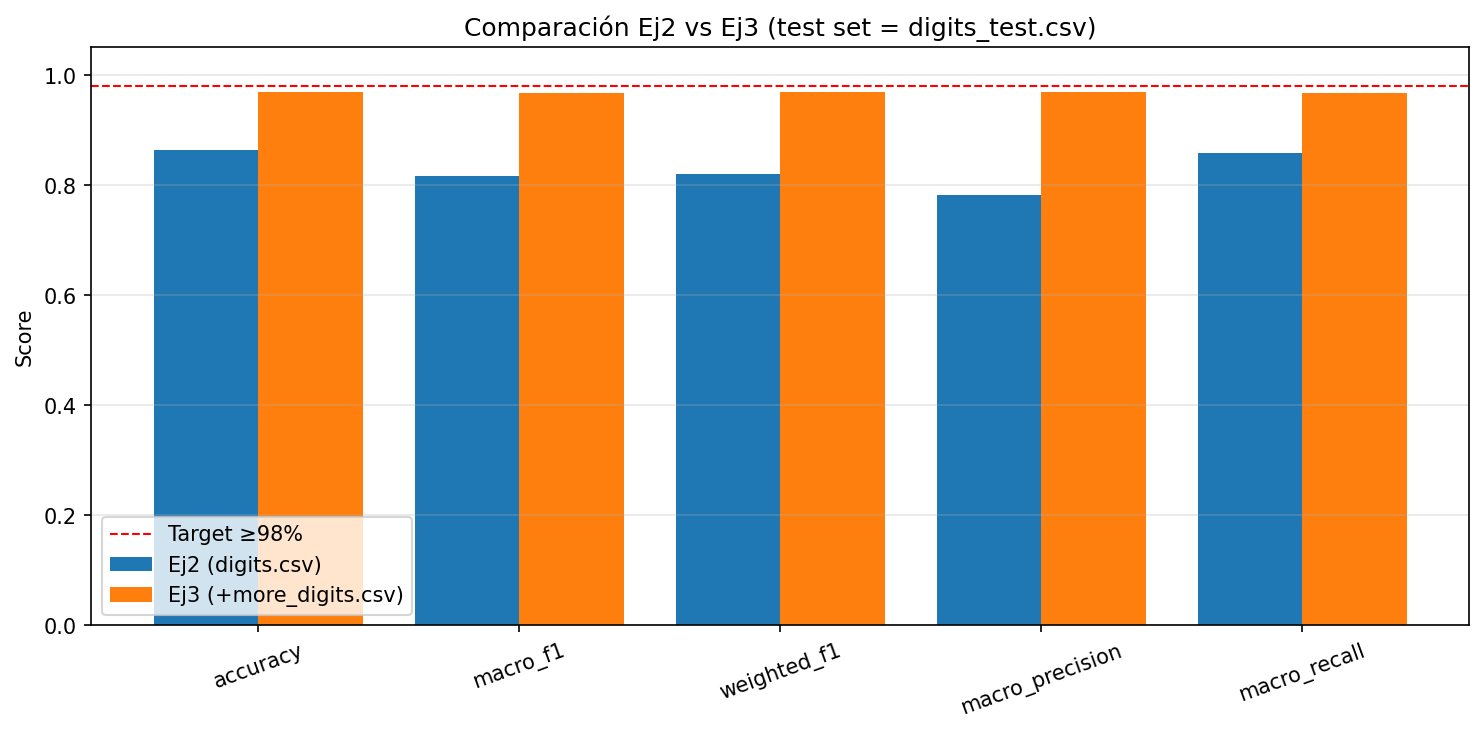
\includegraphics[width=0.72\linewidth]{../../ejercicio3/presentacion/01_comparacion_ej2_vs_ej3.png}\\
\textcolor{muted}{\footnotesize Línea roja: target $\geq 98\%$.}\\[0.4em]

\textbf{El salto principal viene del baseline con extra data}, no de la regularización fina.
\end{frame}

% ============= Curvas Ej3 ganador (ok) =============
\begin{frame}{Ej 3 — Curvas de aprendizaje del modelo ganador}
\centering
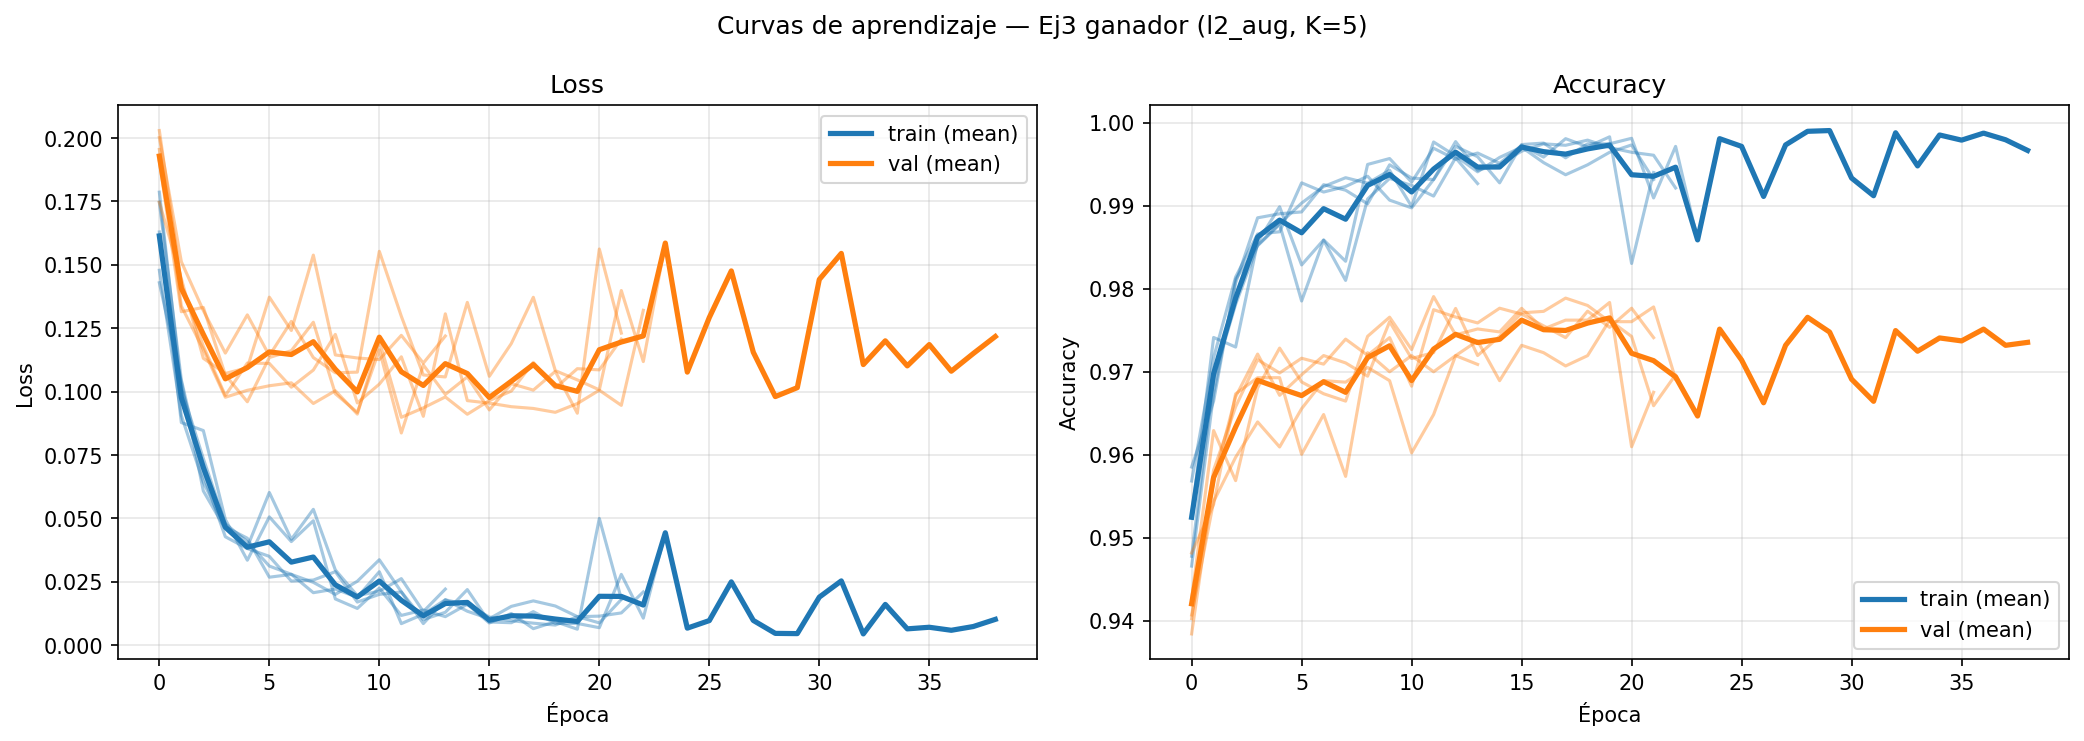
\includegraphics[width=0.78\linewidth]{../../ejercicio3/presentacion/04_curvas_aprendizaje_ej3.png}\\[0.3em]

\textbf{Convergencia más lenta que Ej 2 base} (best\_ep $\sim 10$ vs $5$) por la regularización L2 + augmentation. Sin overfitting visible.
\end{frame}

% ============= Resultados (titulo cambiado de "Análisis: qué movió la aguja" a "Resultados") =============
\begin{frame}{Ej 3 — Resultados: qué ayudó y qué no}
\begin{insight}
\textbf{Lo que ayudó:}
\begin{itemize}
  \item \textbf{Más datos:} \textbf{+10 pp.} El movimiento dominante.
  \item \textbf{L2:} $+0.20$ pp consistente.
  \item \textbf{Aug gaussiana:} $+0.32$ pp \emph{adicional} sobre L2 (sinergia).
\end{itemize}
\end{insight}

\begin{warning}
\textbf{Lo que no ayudó:}
\begin{itemize}\setlength\itemsep{0.1em}
  \item \textbf{Dropout:} gana en val, pierde en test. Reduce varianza al fold, no al shift.
  \item \textbf{wider} \([784,200,100,10]\): mejor en val, peor en test. Descarta falta de capacidad.
  \item \textbf{Combinar todo:} L2+dropout+aug peor que L2+aug solo.
\end{itemize}
\end{warning}
\end{frame}

% ============= Por qué no llegamos al 98% (modificada: conclusiones más simples) =============
\begin{frame}{Ej 3 — Por qué no llegamos al 98\%}
\centering
\Large \textcolor{warn}{\textbf{Mejor: 96.88\%. Faltan 1.12 pp.}}\\[0.8em]

\normalsize\raggedright
\textbf{Hipótesis principal:}
\begin{itemize}\setlength\itemsep{0.3em}
  \item El \textbf{augmentation gaussiano} simula \emph{ruido por píxel}. Pero el shift entre train y test parece ser \emph{geométrico}: distintas personas escriben los dígitos con rotación, desplazamiento y grosor de trazo distintos.
  \item \textbf{El PDF de regularización lista cuatro formas de augmentation; sólo implementamos una} (gaussiano). Faltan rotación, traslación y cambios de escala.
  \item Aumentar la capacidad (\code{wider}) empeoró: \textbf{no es problema de modelo, es problema de cobertura}.
\end{itemize}
\vspace{0.6em}

\begin{takeaway}
\textbf{Próximo paso natural:} augmentation geométrica (rotación / traslación pequeñas).
\end{takeaway}
\end{frame}

% ============= Conclusiones (modificada: "parsimonia" -> "criterio de complejidad") =============
\begin{frame}{Conclusiones del TP}
\textbf{Tres ideas para llevarse:}\\[0.4em]

\begin{enumerate}
  \item \textbf{Una buena pipeline gana más que tunear hiperparámetros.}\\
        El \(+10\)pp del Ej 3 vino de \emph{datos}, no de modelo.
  \item \textbf{Los empates técnicos son más comunes que los wins claros.}\\
        Hay que elegir por \textbf{simplicidad}, tener criterio de complejidad en tiempo y espacio, no solo por pequeñas diferencias de resultados pp.
  \item \textbf{``Mejor en val'' \(\neq\) ``mejor en test'' cuando hay shift.}\\
        Dropout fue el ejemplo de manual: ganador en val, perdedor en test.
\end{enumerate}
\vspace{0.6em}

\centering\small
\begin{tabular}{@{}lc@{}}
\toprule
\textbf{Item} & \textbf{Status} \\
\midrule
Ej 1 — Knowledge distillation + threshold sweep              & \ok \\
Ej 2 — sweeps + final\_eval + análisis del shift             & \ok \\
Ej 3 — \code{more\_digits.csv} + regularización + análisis    & \ok \\
\textbf{Ej 3 — target \(\geq 98\%\)}                          & \nok\ \textbf{(96.88\%)} \\
\bottomrule
\end{tabular}
\end{frame}

% ============= Cierre (modificada: solo "Gracias") =============
{
\setbeamercolor{background canvas}{bg=accent}
\begin{frame}[plain]
\centering
\vspace*{2cm}
\color{white}
{\fontsize{36}{42}\selectfont\bfseries Gracias.}\\[2.5em]

\textcolor{white!75}{\rule{6cm}{0.4pt}}
\end{frame}
}

\end{document}
